\documentclass[10pt]{article}
\usepackage[utf8]{inputenc}
\usepackage[T1]{fontenc}
\usepackage{amsmath}
\usepackage{physics}

\usepackage{amsfonts}
\usepackage{amssymb}
\usepackage[version=4]{mhchem}
\usepackage{stmaryrd}
\usepackage{graphicx}
\usepackage[export]{adjustbox}
\graphicspath{ {./images/} }

\usepackage{listings} % Required for insertion of code
\usepackage{xcolor} % Required for custom colors

% Define custom colors
\definecolor{codegreen}{rgb}{0,0.6,0}
\definecolor{codegray}{rgb}{0.5,0.5,0.5}
\definecolor{codepurple}{rgb}{0.58,0,0.82}
\definecolor{backcolour}{rgb}{0.95,0.95,0.92}

% Setup the style for code listings
\lstdefinestyle{mystyle}{
    backgroundcolor=\color{backcolour},   
    commentstyle=\color{codegreen},
    keywordstyle=\color{magenta},
    numberstyle=\tiny\color{codegray},
    stringstyle=\color{codepurple},
    basicstyle=\ttfamily\footnotesize,
    breakatwhitespace=false,         
    breaklines=true,                 
    captionpos=b,                    
    keepspaces=true,                 
    numbers=left,                    
    numbersep=5pt,                  
    showspaces=false,                
    showstringspaces=false,
    showtabs=false,                  
    tabsize=2
}

% Activate the style
\lstset{style=mystyle}


\title{Ch/ChE 164 Winter 2024 }

\author{}
\date{}


\begin{document}
\maketitle
Midterm

Due Date: Wednesday, February 7, 2024

Midterm Policy

\begin{itemize}
  \item This is an open-book exam. You may look at your notes, your homework, the course notes, and the books listed on the course syllabus.
  \item You may not refer to homework or exams from previous years. You may not consult the internet outside of the course canvas page.
  \item You may take as long as you need before the due date to work on the exam.
  \item You may not consult with one another.
  \item Please write clearly and show all steps; points will be deducted if the midterm is unclear or illegible.
  \item Midterm must be turned in by the end of day on the due date. Late midterm will be penalized $10 \%$ per day unless prior arrangements have been made with the instructor.
\end{itemize}

Some identities that may or may not be useful (not necessarily exhaustive)...

$$
\begin{gathered}
(x+y)^{N}=\sum_{n=0}^{N}\left(\begin{array}{l}
N \\
n
\end{array}\right) x^{n} y^{N-n} \\
(1+x)^{N}=\sum_{n=0}^{N}\left(\begin{array}{l}
N \\
n
\end{array}\right) x^{n}=\sum_{n=0}^{N}\left(\begin{array}{l}
N \\
n
\end{array}\right) x^{n}(1)^{N-n} \\
\frac{1}{1-x}=\sum_{n=0}^{\infty} x^{n} \text { for }|x|<1 \\
\cosh (x)=\frac{e^{x}+e^{-x}}{2}=\frac{d}{d x} \sinh (x) \\
\sinh (x)=\frac{e^{x}-e^{-x}}{2}=\frac{d}{d x} \cosh (x) \\
\tanh (x)=\frac{\sinh (x)}{\cosh (x)}
\end{gathered}
$$
\section{}
\begin{enumerate}
  \item Cross-linking polymer chain (30 pts) Consider polymer chains, each with $N$ monomers, all of which can reversibly associate with any other monomer. For simplicity, let us consider a single polymer chain at temperature $T$.
\end{enumerate}

\begin{center}
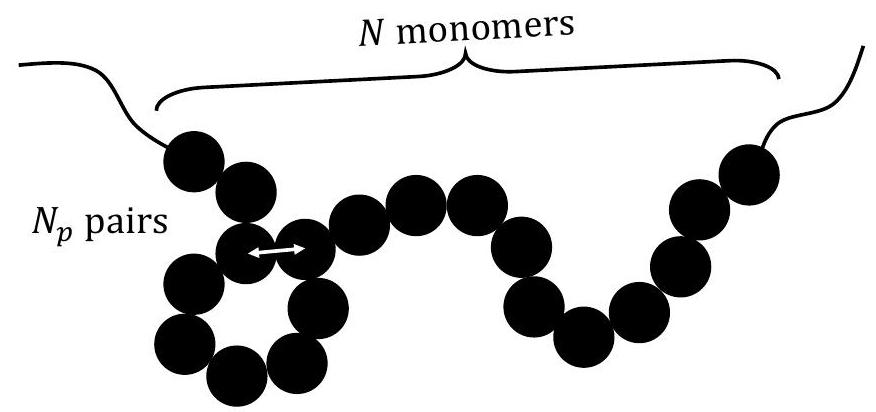
\includegraphics[max width=\textwidth]{2024_02_03_75704bce2caff28cbfb1g-2}
\end{center}

Figure 1: Visualisation of a polymer chain with $N$ monomers forming a single, reversible pair.

(a) (3 pts) How many ways can you select monomers from the chain to form $N_{p}$ pairs?
\subsection{}
 For this part, there will be two variants: one where $N$ is even and one where $N$ is odd. When even, this is:
\begin{equation}
  \binom{N}{2N_p}
\end{equation} 
When odd, this is:
\begin{equation}
  \binom{N-1}{2N_p}
\end{equation}
(b) (5 pts) From these monomers you've selected in 1a, how many ways can you form $N_{p}$ pairs (it may be easier to first consider the case where you can form 2 pairs from 4 monomers)?
\subsection{}
We will start by considering the simple case of forming 2 pairs from 4 monomers:
We can pair the first one with the second one, third one, or fourth one. Because we only have two monomers left unpaired, there are no extra combinatorics associated with this. Now let us consider the case of 6 monomers: Once we establish one pair, the problem reduces to our initial one of forming 2 pairs from 4 monomers. This is a recursive problem. So, for the first pair there are 5 options, then there are only 3 options for the 4 remaining monomers, as discussed previously, and only 1 option for the last pair. So there are $(2N_p -1)!!$ ways to form $N_p$ pairs from $N$ monomers.

Note: You may need to use $(N-1) ! !=(N-1) \times(N-3) \times \ldots$ This can be simplified using: $(N-1) ! !=N ! /\left[(N / 2) ! 2^{N / 2}\right]$.

(c) $(6$ pts) The product from $\mathbf{1 a}$ and $\mathbf{1} \mathbf{b}$ will give you the microcanonical partition function for a system with $N_{p}$ pairs as:

$$
\Omega\left(N, N_{p}\right)=\frac{N !}{\left(N-2 N_{p}\right) ! N_{p} ! 2^{N_{p}}}
$$

If the energetic gain from forming a single pair is $-\epsilon$, write out the canonical partition function, $Q(N, T)$, for this system. You should end up with a sum over all possible values of $N_{p}$.
\subsection{}
The canonical partition function would be given by:
\begin{equation}
  Q(N, T) = \sum_{N_p=0}^{N/2} \Omega(N, N_p) e^{-\beta \epsilon N_p}
\end{equation}
Inserting the expression for $\Omega(N, N_p)$, we get:
\begin{equation}
  Q(N, T) = \sum_{N_p=0}^{N/2} \frac{N !}{\left(N-2 N_{p}\right) ! N_{p} ! 2^{N_{p}}} e^{-\beta \epsilon N_p}
\end{equation}
\\
(d) $(10$ pts) Find the most-probable term in this sum, and show that the corresponding value for the fraction of monomers associated $\left(p=2 N_{p} / N\right)$ is given by:
$$
p=1+\frac{\frac{\exp (-\beta \epsilon)}{N}-\sqrt{\left(2+\frac{\exp (-\beta \epsilon)}{N}\right)^{2}-4}}{2}
$$
\subsection{}
An arbitrary term in the sum is given by:
\begin{equation}
  t_{N_p} = \frac{N !}{\left(N-2 N_{p}\right) ! N_{p} ! 2^{N_{p}}} e^{-\beta \epsilon N_p}
\end{equation}
We can find the most-probable term by taking the derivative of $t_{N_p}$ with respect to $N_p$ and setting it equal to zero. Or alternatively, we can choose to maximize the logarithm of $t_{N_p}$, which is equivalent, so the first derivative of the logarithm of $t_{N_p}$ with respect to $N_p$ is zero:
\begin{equation}
  \frac{d}{dN_p} \ln(t_{N_p}) = 0
\end{equation}
The logarithm of $t_{N_p}$ is given by:
\begin{equation}
  \ln(t_{N_p}) = \ln(N!) - \ln((N-2N_p)!) - \ln(N_p!) - N_p \ln(2) - \beta \epsilon N_p
\end{equation}
% We Taylor expand this around the most-probable value of $N_p$, which we will call $N_p^*$ (already simplifying since we know the first derivative is zero at this point). Also, we define $t_{N_p^*}$ as $t_{N_p}$ evaluated at $N_p^*$. We get:
% \begin{equation}
%   \ln(t_{N_p}) \approx \ln(t_{N_p^*}) + \frac{1}{2} \pdv[2]{\ln(t_{N_p})}{N_p} \bigg|_{N_p=N_p^*} (N_p - N_p^*)^2+ \ldots
% \end{equation}
% We
Using Stirling's approximation, we can simplify the logarithm of $t_{N_p}$ to:
\begin{equation}
  \ln(t_{N_p}) \approx N \ln(N) - (N-2N_p) \ln(N-2N_p) - N_p \ln(N_p) - N_p \ln(2) - \beta \epsilon N_p
\end{equation}
We can now take the first derivative of this with respect to $N_p$ and set it equal to zero:
\begin{equation}
  0 = - \beta \epsilon - \log{\left(N_p \right)} + 2 \log{\left(N - 2 N_p \right)} - \log{\left(2 \right)} + 1
\end{equation}
Bring the non-logarithmic terms to the left-hand side:
\begin{equation}
  \beta \epsilon - 1 = - \log{\left(N_p \right)} + 2 \log{\left(N - 2 N_p \right)} - \log{\left(2 \right)}
\end{equation}
Exponentiate both sides:
\begin{equation}
  \exp{\left(\beta \epsilon - 1 \right)} = \frac{(N - 2 N_p)^2}{2N_p}
\end{equation}
Solving for $N_p$:
\begin{equation}
  N_p = \frac{2 e N - \sqrt{\left(4 e N + e^{\beta \epsilon}\right) e^{\beta \epsilon}} + e^{\beta \epsilon}}{4 e}
\end{equation}

(e) (6 pts) Let us now consider the limits of the fraction of monomers associated. Consider both the limit at high $(\beta \rightarrow 0)$ and low $(\beta \rightarrow \infty)$ temperatures. In terms of energetic interactions and conformational contributions, which effect dominates in either limit?
\subsection{}
We want to consider the term:
\begin{equation}
  p=1+\frac{\frac{\exp (-\beta \epsilon)}{N}-\sqrt{\left(2+\frac{\exp (-\beta \epsilon)}{N}\right)^{2}-4}}{2}
\end{equation}
At high temperatures, $\beta \rightarrow 0$, the exponential term in the numerator becomes $\frac{1}{N}$. We expand the numerator with this:
\begin{equation}
  p=1+\frac{\frac{1}{N}-\sqrt{\left(2+\frac{1}{N}\right)^{2}-4}}{2} = 1+\frac{\frac{1}{N}-\sqrt{4+4\frac{1}{N}+\frac{1}{N^2}-4}}{2} = 1+\frac{\frac{1}{N}-\sqrt{4\frac{1}{N}+\frac{1}{N^2}}}{2}
\end{equation}


\section*{2. A diluted magnetic fluid ( $30 \mathrm{pts}$ )}
Consider a lattice with $N$ lattice sites and $n$ spins in an external magnetic field $H$ that is pointing up. The lattice need not have every site filled with a spin.

\begin{itemize}
  \item Spins can be either up or down, corresponding to $s_{i}=+1$ and $s_{i}=-1$. Spins aligned parallel to the field have an energy $-H$ whereas spins antiparallel have energy $H$.
  \item Vacant sites have no spin and thus no interaction with a magnetic field.
\end{itemize}

You can think of this as a crude model for a paramagnetic fluid that has some non-magnetic impurities. The lattice is connected to a reservoir at temperature $T$ and chemical potential $\mu$ such that energy $E$ and number of spins $n$ are allowed to fluctuate. We can call this a constrained grand canonical ensemble because the particle number $(n)$ can fluctuate, but cannot exceed $N$ since the lattice has a fixed number of sites. In this case $N$ acts like $V$ because $V=N v_{\text {site }}$ where $v_{\text {site }}$ is just the volume of a single lattice site.

\begin{center}
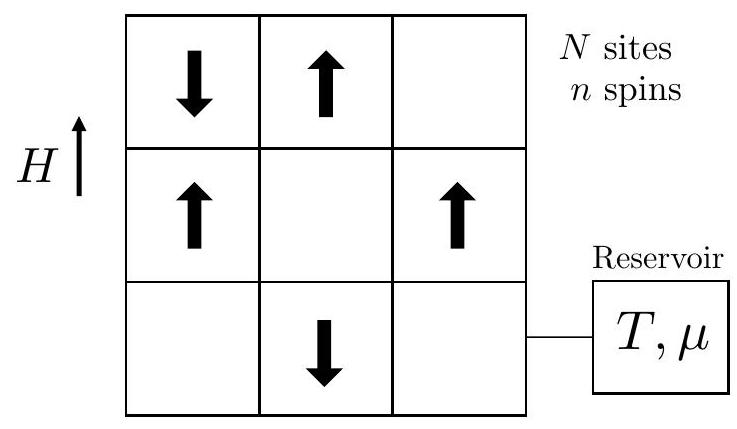
\includegraphics[max width=\textwidth]{2024_02_03_75704bce2caff28cbfb1g-3}
\end{center}

Figure 2: System schematic for the diluted paramagnetic fluid. The example here is showing the case for $N=9$ and $n=5$. Note that $n$ fluctuates by exchanging with the reservoir.

(a) (2 pts) What are the definitions of microstate and macrostate for this system?
\subsection{}
The microstate is a specific configuration of the lattice, where each site is either filled with a spin or is vacant. The macrostate is a collection of microstates that have the same energy and number of spins.

(b) ( 8 pts) Derive the closed-form grand canonical partition function $\Xi(N, T, \mu, H)$.

Start from either equality below

$$
\Xi(N, T, \mu, H)=\sum_{\nu} e^{-\beta E_{\nu}+\beta \mu n_{\nu}}=\sum_{n} Q(N, T, n, H) e^{\beta \mu n}
$$

and show that

$$
\Xi(N, T, \mu, H)=\left[1+2 e^{\beta \mu} \cosh (\beta H)\right]^{N}
$$

There are multiple ways to do this!
\subsection{}
At each site there are 3 possibilities: the site could be vincent, giving an energy of 0, the spin could be aligned with the field, giving an energy of $-H$, or the spin could be antiparallel to the field, giving an energy of $H$. The partition function for a single site is then:
\begin{equation}
  Q_{\text{site}} = 1 + e^{\beta \mu} e^{-\beta H} + e^{\beta \mu} e^{\beta H}
\end{equation}
We can factor out the $e^{\beta \mu}$ from the last two terms and multiply them by$\frac{2}{2}$:
\begin{equation}
  Q_{\text{site}} = 1 + 2 e^{\beta \mu}\left( \frac{e^{-\beta H} + e^{\beta H}}{2} \right)
\end{equation}
We can recognize the term in the parentheses as the hyperbolic cosine:
\begin{equation}
  Q_{\text{site}} = 1 + 2 e^{\beta \mu} \cosh(\beta H)
\end{equation}
This is a partition function for a single site, so for all $N$ sites, we get:
\begin{equation}
  \Xi(N, T, \mu, H) = \left[1 + 2 e^{\beta \mu} \cosh(\beta H) \right]^N
\end{equation}
(c) (6 pts) Solve for the average fraction of occupied sites in the system $\langle x\rangle=\langle n\rangle / N$ using an appropriate derivative. What happens as $H \rightarrow \infty$ ? Explain the physical intuition of the limiting behavior.
\subsection{}
The relevant thermodynamic potential is the grand free energy, $W = -kT \ln(\Xi)$. in its deferential form, this is given by:
\begin{equation}
  dW = -S dT - P dV - N d\mu - M dH
\end{equation}
So, if we want to solve for the average value of $n$, we can take the negative derivative of $W$ with respect to $\mu$, or equivalently, the derivative of $\ln(\Xi)$ with respect to $\beta\mu$. We get:
\begin{equation}
  \pdv{\ln(\Xi)}{\mu} = \frac{N}{1+2e^{\beta\mu}\cosh(\beta H)} \times 2\beta e^{\beta\mu}\cosh(\beta H)
\end{equation}
Dividing by $N$ and $\beta$:
\begin{equation}
  \langle x \rangle = \left( \frac{2e^{\beta\mu}\cosh(\beta H)}{1+2e^{\beta\mu}\cosh(\beta H)} \right)
\end{equation}
The limit of $\cosh(x)$ as $x \rightarrow \infty$ is $\frac{e^x}{2}$, or $\infty$. So, as $H \rightarrow \infty$, the fraction of occupied sites approaches 1. This makes sense, as many sites will want to have spins that align with the field to minimize their energy.\\
(d) (3 pts) In the reservoir, we have $H=0$. If we also know that the fraction of sites occupied in the reservoir is $x_{R}$, then what is $e^{\beta \mu}$ ?
\subsection{}
If in the reservoir, $H=0$, then $\cosh(\beta H) = 1$. So the fraction of occupied sites in the reservoir is given by:
\begin{equation}
  x_R = \frac{2\beta e^{\beta\mu}}{1+2e^{\beta\mu}}
\end{equation}
Solving for $e^{\beta\mu}$:
\begin{equation}
  e^{\beta\mu} = \frac{x_{R}}{2 \left(\beta - x_{R}\right)}
\end{equation}
% Inline Python code in the document
\begin{lstlisting}[language=Python]
from sympy import *
# divine the symbols of the equation x_R = \frac{2\beta e^{\beta\mu}}{1+2e^{\beta\mu}}
x_R, beta, mu = symbols('x_R beta mu')
eq = Eq(x_R, 2*beta*exp(beta*mu)/(1+2*exp(beta*mu)))
# solve for e^{\beta\mu}
solution = solve(eq, exp(beta*mu))
print(latex(solution[0].simplify()))
\end{lstlisting}
(e) (4 pts) Calculate the average magnetisation $\langle M\rangle$.

Note the differential form of the grand free energy including the magnetisation

$$
d W=-S d T-P v_{\text {site }} d N-n d \mu-M d H
$$
\subsection{}
The average magnetisation is given by the derivative of the grand free energy with respect to $H$:
\begin{equation}
  \langle M \rangle = -\pdv{W}{H} = \frac{1}{\beta } \pdv{\ln(\Xi)}{H}
\end{equation}
This derivative is given by:
\begin{equation}
  \pdv{\ln(\Xi)}{H} = \frac{2 N \beta e^{\beta \mu} \sinh{\left(H \beta \right)}}{2 e^{\beta \mu} \cosh{\left(H \beta \right)} + 1}
\end{equation}
% Inline Python code in the document
\begin{lstlisting}[language=Python]
from sympy import symbols, diff, cosh, exp, ln, latex, simplify

# Define the symbols
beta, mu, H, N = symbols('beta mu H N')

# Define the grand canonical partition function
Xi = (1 + 2*exp(beta*mu)*cosh(beta*H))**N

# Compute the natural logarithm of the partition function
ln_Xi = ln(Xi)

# Perform the differentiation of ln(Xi) with respect to mu
dlnXi_dH = diff(ln_Xi, H)

print(latex(dlnXi_dH.simplify()))

\end{lstlisting}
Dividing by $\beta$:
\begin{equation}
  \langle M \rangle = \frac{2N e^{\beta \mu} \sinh{\left(H \beta \right)}}{2 e^{\beta \mu} \cosh{\left(H \beta \right)} + 1}
\end{equation}
(f) (3 pts) Calculate the magnetic susceptibility, $\chi=(\partial\langle M\rangle / \partial H)_{T, N, \mu}$.
\subsection{}
The magnetic susceptibility is given by the derivative of the average magnetisation with respect to $H$:
\begin{equation}
  \chi = \pdv{\langle M \rangle}{H} =  \frac{2 N \beta \left(2 e^{\beta \mu} + \cosh{\left(H \beta \right)}\right) e^{\beta \mu}}{\left(2 e^{\beta \mu} \cosh{\left(H \beta \right)} + 1\right)^{2}}
\end{equation}
% Inline Python code in the document
\begin{lstlisting}[language=Python]
from sympy import *
# Define the symbols for \langle M \rangle = \frac{2N e^{\beta \mu} \sinh{\left(H \beta \right)}}{2 e^{\beta \mu} \cosh{\left(H \beta \right)} + 1}
N, beta, mu, H = symbols('N beta mu H')
M = 2*N*exp(beta*mu)*sinh(H*beta) / (2*exp(beta*mu)*cosh(H*beta) + 1)
# take the deviate with respect to H
dM_dH = diff(M, H)
print(latex(dM_dH.simplify()))
\end{lstlisting}
(g) (4 pts) Relate the susceptibility $\chi$ to the fluctuations in magnetisation $\sigma_{M}^{2}$. How does $\sigma_{M} /\langle M\rangle$ scale with $N$ ? This should require little additional work!

\section*{3. Simple Elastic Molecule under Fixed Tension (40 pts)}
A crude way to treat a rubber band is by treating it as a chain of linked segments that can take configurations of different lengths. In general we could also assume that the different configurations have different energies.

Assume that there are $N$ total distinguishable segments which each have access to two different conformations: type $\mathbf{A}$ and type $\mathbf{B}$. The types are distinguished by their length and their energy.

\begin{itemize}
  \item Type A has length $a$ and energy $\epsilon_{a}$.
  \item Type B has length $b$ and energy $\epsilon_{b}$.
\end{itemize}

\begin{center}
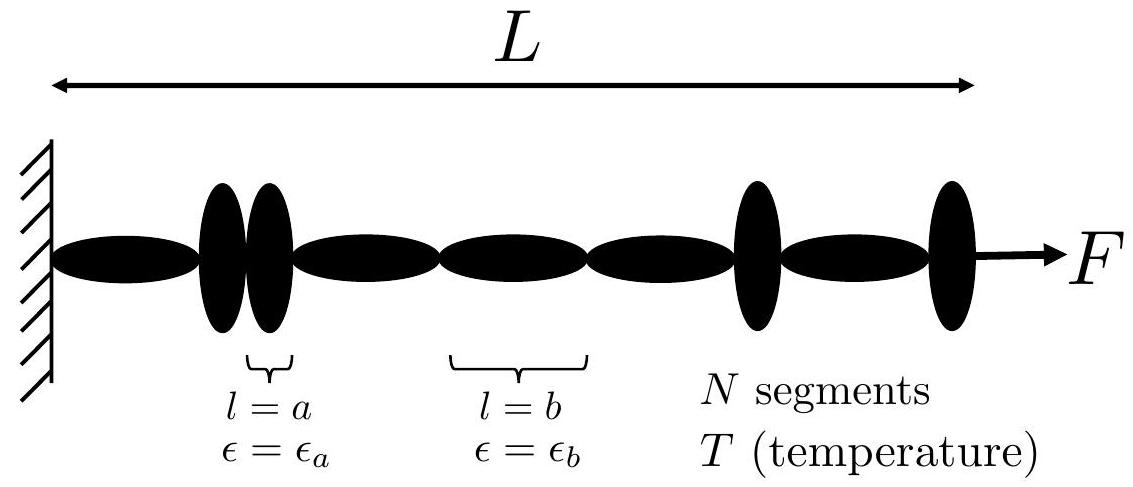
\includegraphics[max width=\textwidth]{2024_02_03_75704bce2caff28cbfb1g-5}
\end{center}

Figure 3: Schematic for the elastic molecule. Note that in this case $L$ can fluctuate by changing segment conformations (not by changing $N$ ). The specific example shown is for $N=9$ and $L=4 a+5 b$.

(a) $(8$ pts) The molecule is placed in a bath at temperature $T$ and extended with a fixed force $F$. Starting from the Euler equation for the relevant free energy at fixed $(N, F, T)$, use the variational method to derive the probability distribution $P_{\nu}(N, F, T)$ and show that the partition function $Z(N, F, T)$ in this ensemble is given by:

$$
Z(N, F, T)=\sum_{\nu} e^{\beta F L_{\nu}} e^{-\beta E_{\nu}}
$$

Note that the Euler equation and fundamental equation for the internal energy are, respectively:

$$
\begin{gathered}
E=T S+F L+\mu N \\
d E=T d S+F d L+\mu d N
\end{gathered}
$$

(b) (6 pts) Using the answer to part (a), show that the partition function in the ( $N, F, T)$ ensemble is given by

$$
Z(N, F, T)=\left[e^{\beta F a} e^{-\beta \epsilon_{a}}+e^{\beta F b} e^{-\beta \epsilon_{b}}\right]^{N}
$$

We will now look at a specific case, that yields some very interesting results. Let's take the simplest example, where $\epsilon_{a}=\epsilon_{b}=0$ and $a=0$. Thus, each segment is either vertical (and has no length) or is horizontal (and has length $b$ ). In this case, the partition function simplifies to,

$$
Z(N, F, T)=\left[1+e^{\beta F b}\right]^{N}
$$

(c) (4 pts) Calculate the extension-force equation of state, $\langle L\rangle=L(N, F, T)$.

$$
\langle L\rangle=N b \frac{e^{\beta F b}}{1+e^{\beta F b}}
$$

(d) (4 pts) Find the equilibrium length $\left(L_{0}\right)$ of the molecule at zero tension (i.e. at $F=0$ ). Does this answer make sense? Why or why not?

(e) (6 pts) Now we will derive Hooke's law and calculate the spring constant using statistical mechanics!

i. Invert $L(N, F, T)$ to get the force-extension equation of state, $F(\langle L\rangle, N, T)$.

ii. Taylor expand $F(\langle L\rangle, N, T)$ out to first order around the equilibrium chain length from 3d. Physically, when does this approximation apply?

iii. Extract the spring constant $K_{s}$ by inspection.

(f) (4 pts) Relate the fluctuations in length $\sigma_{L}^{2}$ at $F=0$ to the spring constant, $K_{s}$. Explain why this relationship physically makes sense.

(g) (8 pts) For this more simplified model of the chain where each segment is either vertical or horizontal, we can analyze the behavior using a fixed energy and length ensemble (i.e. the microcanonical ensemble). The partition function is given by $\Omega(N, L, E)$.

i. Calculate the microcanonical partition function at length $L=n b$, where $n$ is the number of horizontal segments.

ii. Show that your answer to $\mathbf{3 d}$ maximizes the entropy.

iii. Verify that you obtain the same force-extension equation of state $F(N, L, T)$ in this ensemble.


\end{document}